\documentclass[10pt,a4paper,twocolumn]{article}

\usepackage{microtype,nowidow}
\usepackage{fontenc,newtxtext}
\usepackage[left=1.5cm,right=1.5cm,top=2cm,bottom=2cm]{geometry}

\usepackage{amsmath, amssymb, bm}
\usepackage{graphicx}
\usepackage{booktabs}
\usepackage{hyperref}
\usepackage{cleveref}
\usepackage[backend=biber]{biblatex}
\addbibresource{references.bib}

\usepackage{macros}

\title{\bfseries Approximate inference for Bayesian neural networks}
\author{Silas Brack}
\date{Spring 2022}

\begin{document}
\maketitle

\begin{abstract}
\end{abstract}

\section{Introduction}

Neural networks (NNs) suffer from calibration issues and overconfidence, catastrophic interference in continual learning, and sensitivity to hyper-parameter selection.

Bayesian neural networks (BNNs) arise from applying Bayesian inference on the layer weights of NNs and are one solution for these issues, allowing an estimate of the uncertainty of the output of NNs.

However, BNNs networks are expensive and cumbersome to train.
Their posteriors are intractable in an exact sense, meaning these have to be approximately inferred.
Furthermore, they inherit having a large parameter space (and consequently a large optimisation space) from their non-Bayesian counterparts, leading to slow inference for traditional methods such as Markov-chain Monte Carlo (MCMC), which, while yielding very competitive results~\cite{izmailov2021bayesian}, scales poorly with increasing dimensionality.
Other Bayesian and quasi-Bayesian methods have been proposed as alternatives, such as variational inference, SWAG/MultiSWAG, deep ensembles, and Laplace approximations.

This paper analyses these alternative approximate inference methods.

\section{Previous Work}\label{sec:priorwork}

\subsection{Bayes’ Theorem}

Bayes' theorem describes the probability of an event occurring with respect to prior knowledge of that event.
Specifically for modelling, it can be used to relate latent variables with observed variables, allowing distributions on these latent variables to be inferred.
We therefore want to find the posterior \(p(\bm \theta \given \bm y)\) by
According to Bayes' theorem, the posterior is given by
\begin{align}\label{eq:bayes}
    p(\bm \theta \given \bm y) = \frac{p(\bm y \given \bm \theta) p(\bm \theta)}{p(\bm y)}
\end{align}
where \(p(\bm y \given \bm \theta)\) is the likelihood, parameterised by the model parameters \(\bm \theta\), \(p(\bm \theta) = p(\bm \theta; \bm \alpha)\) is the prior, parameterised by its hyper-parameters \(\bm \alpha\), and \(p(\bm y) = p_{\bm \theta}(\bm y)\) is the marginal likelihood (or evidence).

Furthermore, the posterior predictive probability, i.e., the probability of observing some new data, is given by
\begin{align}
    p(\bm y_{\mathrm{new}} \given \bm y) = \int p(\bm y_{\mathrm{new}} \given \bm \theta) p(\bm \theta \given \bm y)\,d\bm\theta.
\end{align}

\subsection{Variational Inference}

In variational inference (VI), we minimise the KL divergence between the posterior distribution \(p(\bm \theta \given \bm y)\) and a variational distribution \(q_{\bm \phi}(\bm \theta)\) parameterised by its variational parameters \(\bm \phi\) by optimising with respect to these parameters.
The KL divergence is defined as
\begin{align}
    \kld{q(\bm \theta)}{p(\bm y \given \bm \theta)} \equiv{} & \E{q}{\log \frac{q(\bm \theta)}{p(\bm y \given \bm \theta)}} \label{eq:kld}  \\
    ={}                                                      & \E{q}{\log q(\bm \theta)} - \E{q}{\log p(\bm y \given \bm \theta)} \nonumber
\end{align}
However, the KL divergence contains the evidence term \(\log p(\bm y)\), which is intractable.
Instead, we define a lower bound on this marginal likelihood term that is surrogate to the KL divergence (known as the ELBO).
Since they are surrogate, ELBO fulfils the property \(\elbo = \log p(\bm y) - \kld{q(\bm \theta)}{p(\bm y \given \bm \theta)}\), minimising the KL divergence is equivalent to maximising the ELBO, which is defined as
\begin{align}
    \elbo \equiv{} & \E{q}{\log p(\bm y, \bm \theta)} - \E{q}{\log q(\bm \theta)} \nonumber                                                                                                               \\
    ={}            & \E{q}{\log p(\bm y \given \bm \theta)} + \E{q}{\log p(\bm \theta)} - \E{q}{\log q(\bm \theta)} \nonumber                                                                             \\
    ={}            & \E{q}{\log p(\bm y \given \bm \theta)} - \underbrace{- \E{q}{\log p(\bm \theta)}}_{\text{Cross-entropy}} + \underbrace{- \E{q}{\log q(\bm \theta)}}_{\text{Entropy}} \label{eq:elbo}
\end{align}
where the first term \(\E{q}{\log p(\bm y \given \bm \theta)}\) is the data (or likelihood) term, \(-\E{q}{\log p(\bm \theta)}\) is the cross-entropy of the prior with respect to the variational approximation, and \(-\E{q}{\log q(\bm \theta)}\) is the entropy term of the variational approximation.
The last two terms can be interpreted as the regularising KL divergence (or relative entropy) from the prior to the variational approximation, \(\kld{q(\bm \theta)}{p(\bm \theta)} = \E{q}{\log q(\bm \theta)} - \E{q}{\log p(\bm \theta)}\).
Furthermore, the likelihood term in the ELBO can be decomposed further by assuming independence in the observations as \(\E{q}{\log p(\bm y \given \bm \theta)} = \frac{1}{N} \sum^N_i \E{q}{\log p(y_i \given \bm \theta)}\).

Overall BNNs have been found to be relatively ineffective unless the number of observations is greater than the number of model parameters.\emph{Source?}

\subsection{Methods}\label{ssec:methods}

Multiple approximate inference methods were implemented.
Specifically, \emph{maximum a posteriori} estimation, Laplace approximation, VI with mean-field, full-rank, low-rank and radial variational families, deep ensembles, and MultiSWAG.
These methods will be described in the following sections.

\subsubsection{Maximum a Posteriori Estimation}

\emph{Maximum a posteriori} estimation finds a point estimate of the posterior given by its maximum.
It can therefore be interpreted as a Delta distribution estimate of the posterior \(p(\bm \theta \given \bm y) \approx \delta(\bm \theta_\mathrm{MAP})\), where \(\bm \theta_{\text{MAP}}\) is defined as
\begin{align}
    \bm \theta_\mathrm{MAP}
    ={} & \max_{\bm \theta} p(\bm \theta \given \bm y) \nonumber                                            \\
    ={} & \max_{\bm \theta} \log p(\bm \theta \given \bm y) \nonumber                                       \\
    ={} & \max_{\bm \theta} \left[ \log p(\bm y \given \bm \theta) + \log p(\bm \theta) \right] \nonumber   \\
    ={} & \max_{\bm \theta} \left[ \sum_{i=1}^N \log p(y_i \given \bm \theta) + \log p(\bm \theta) \right].
\end{align}
As an optimisation problem, maximising the posterior corresponds to minimising the regularised loss,
\begin{align}
    \bm \theta_{\text{MAP}} ={} & \arg \min_{\bm \theta} \mathcal{L}(\bm y; \bm \theta)                                                   \\
    ={}                         & \arg \min_{\bm \theta} \left[ -\sum_{i=1}^N \log p(y_i \given \bm \theta) - \log p(\bm \theta) \right].
\end{align}
In this formulation, the term \(-\sum_{i=1}^N \log p(y_i \given \bm \theta)\) is known as the empirical loss or reconstruction loss and the term \(\log p(\bm \theta)\) is the regulariser.

\subsubsection{Laplace Approximation}

In the Laplace approximation (LA)~\cite{daxberger2021laplace}, the posterior is approximated by a Gaussian, similarly to mean-field VI.
However, instead of finding the optimal Gaussian distribution locations and scales by maximising the ELBO, the LA finds the location by computing the MAP solution \(\bm \theta_{\text{MAP}}\) and the scale by approximating the log posterior with a second degree Taylor expansion around this solution (\(\bm \theta_0 = \bm \theta_{\text{MAP}}\)) and determining the curvature via its Hessian matrix \(\bm H = \left.\nabla^2_{\bm \theta} \log p(\bm \theta \given \bm y) \right|_{\bm \theta_\mathrm{MAP}}\).
Since the Taylor expansion is performed around the MAP solution, the first order derivative is zero, and the expansion is simply given by
\begin{align}
    \ln p(\bm \theta \given \bm y) \approx{}     & \ln p(\bm \theta_0 \given \bm y)        + \frac{1}{2} (\bm \theta - \bm \theta_0)\T \bm H (\bm \theta - \bm \theta_0)                        \label{eq:laplace-taylor} \\
    \tilde{p}(\bm \theta \given \bm y) \approx{} & p(\bm \theta_0 \given \bm y) \exp\left(-\frac{1}{2} (\bm \theta - \bm \theta_0)\T \bm H (\bm \theta - \bm \theta_0)\right).\nonumber
\end{align}
Normalising this unnormalised posterior yields the Laplace approximation of the posterior
\begin{align}
    p(\bm\theta \given \bm y) \approx{} & \sqrt{\frac{\det\bm H}{(2 \pi)^D}} \exp\left(-\frac{1}{2} (\bm \theta - \bm \theta_0)\T \bm H (\bm \theta - \bm \theta_0)\right) \nonumber \\
    \approx{}                           & \normal(\bm \theta_0, \bm H^{-1}) = \normal(\bm \theta_{\text{MAP}}, \bm H^{-1}).\label{eq:laplace}
\end{align}

\subsubsection{Mean-Field Variational Approximation}\label{ssec:mfvi}

One common variational family used to approximate the real posterior is a product of independent Gaussian distributions (the mean-field approximation) such that each model parameter is sampled from a normal distribution and is independent of all other model parameters, yielding a Gaussian with a diagonal covariance matrix.
In mean-field VI, model weights are sampled from an approximate posterior \(q(\bm \theta) \approx p(\bm{\theta} \given \bm y)\) as
\begin{align}
    q(\bm \theta) ={} & \normal(\bm \mu, \bm \sigma) \Leftrightarrow \nonumber         \\
    \bm{\theta} ={}   & \bm{\mu} + \bm{\sigma} \circ \bm{\epsilon}\label{eq:meanfield}
\end{align}
where \(\bm{\epsilon} \sim \normal(\bm 0, \identity)\).
For this type of variational approximation, the entropy term is given by \(\entropy{q(\theta)} = - \sum_i \log \sigma_i\) and the cross-entropy of the prior relative to the variational approximation is calculated via Monte Carlo simulation by taking the prior log probability with respect to mean-field posterior samples as
\begin{align}
    \crossentropy{q(\bm\theta)}{p(\bm\theta)} ={} & - \int q(\bm\theta) \log(p(\bm\theta))\,d\bm\theta \nonumber \\
    \approx{}                                     & \frac{1}{S} \sum^S_{s=1} \log p(\bm{\theta}^{(s)})
\end{align}
where \(\bm{\theta}^{(s)} \sim \normal(\bm{\mu}, \bm{\sigma})\).

The use of the mean-field approximation for BNNs has been found to be unreliable~\cite{wu2018deterministic} and, for increasingly wide neural networks, converges towards the prior~\cite{coker2021wide}.
However, for \emph{deep} BNNs, the mean-field assumption may be reasonable~\cite{farquhar2020liberty}.

\subsubsection{Full-Rank Variational Approximation}

As an alternative to the mean-field approximation, a full-rank approximation doesn't assume independence of the model parameters, instead being sampled as
\begin{align}\label{eq:fullrank}
    q(\bm \theta) = \normal(\bm \mu, \bm \Sigma_{\mathrm{FR}}).
\end{align}
For \(D\) model parameters, while a mean-field approximation has scale parameters \(\bm \sigma^D\), the full-rank approximation has scale parameters \(\bm \Sigma_{\mathrm{FR}}^{D \times D}\).
The variational parameters scale quadratically with the number of model parameters, which constitutes a significant limitation of this type of approximation.
Specifically, since NNs are typically overparameterised, possessing from thousands to millions to billions of parameters, the quadratic number of variational parameters makes this type of VI infeasible for BNNs.
As such, full-rank VI is not applied in any of the experiments in this paper.

\subsubsection{Low-Rank Variational Approximation}

As a compromise between the last two methods, a low-rank variational approximation uses a low-rank approximation of the covariance matrix \(\bm \Sigma_{\mathrm{LR}}\).
\begin{align}\label{eq:lowrank}
    q(\bm \theta) = \normal(\bm \mu, \bm \Sigma_{\mathrm{LR}}).
\end{align}
This approximation is obtained by reconstructing a covariance matrix paremeterised by the covariance factor \(\tilde{\bm \Sigma}\) and diagonal element vector \(\bm \sigma_{\text{diag}}\) as
\begin{align}
    \hat{\bm \Sigma}_{\text{LR}} = \tilde{\bm \Sigma} \tilde{\bm \Sigma}\T + \bm \sigma_{\text{diag}} \nonumber \\
    \bm \Sigma_{\text{LR}} = \min_{\hat{\bm \Sigma}_{\text{LR}}} \norm{\bm \Sigma - \hat{\bm \Sigma}_{\text{LR}}}_F \label{eq:lowrank-covariance}
\end{align}

\subsubsection{Radial Variational Approximation}

\textcite{farquhar2020radial} introduces the Radial approximate posterior,
For each NN layer, this posterior is sampled similarly to the mean-field (\cref{eq:meanfield}), but by normalising the \(\bm{\epsilon}\) term (projecting it onto a hypersphere) yielding a direction term \(\bm{\epsilon}/\norm{\bm{\epsilon}}\), and scaling it by the distance \(r\).
Therefore, for each layer, the radial posterior is sampled as
\begin{align}\label{eq:radial}
    q(\bm \theta) ={} & \mathrm{Radial}(\bm{\mu}, \bm{\sigma}) \nonumber                          \\
    \bm{\theta} ={}   & \bm{\mu} + \bm{\sigma} \circ \frac{\bm{\epsilon}}{\norm{\bm{\epsilon}}} r
\end{align}
where \(\bm{\epsilon} \sim \normal(\bm{0}, \identity)\), \(r \sim \normal(0, 1)\).
The entropy term of the Radial approximate posterior is given
\(\entropy{q(\theta)} = - \sum_i \log \sigma_i + \mathrm{const}\) (and is therefore approximately equal to the entropy of the mean-field approximation up to a constant) and the cross-entropy term is calculated via Monte Carlo simulation as for mean-field VI (\cref{ssec:mfvi}), but by sampling from a radial posterior \(\bm{\theta}^{(s)} \sim \mathrm{Radial}(\bm{\mu}, \bm{\sigma})\) as in \cref{eq:radial}.

\subsubsection{Deep Ensembles}

In deep ensembles~\cite{lakshminarayanan2017simple}, \(M\) neural networks are trained with different initialisations.
In this way, multiple local MAP solutions \(\bm\theta^{(m)}\) are obtained and equally considered, such that \(p(\bm \theta = \bm \theta^{(m)} \given \bm y) = 1 / M\) for every \(\bm \theta^{(m)} \in \{\bm\theta^{(1)}, \ldots, \bm\theta^{(M)}\}\) (and 0 elsewhere).
To make predictions with a deep ensemble, we use the posterior predictive given by
\begin{align}
    p(\bm y_{\mathrm{new}} \given \bm y)
    ={} & \int p(\bm y_{\mathrm{new}} \given \bm \theta) p(\bm \theta \given \bm y)\,d\bm\theta \nonumber \\
    ={} & \frac{1}{M} \sum_{m=1}^M p(\bm y_{\mathrm{new}} \given \bm\theta^{(m)})
\end{align}
where \(p(\bm y_{\mathrm{new}} \given \bm\theta^{(m)})\) are the normalised logits, or predicted probabilities, from model \(m\) in the ensemble.

\subsubsection{MultiSWAG}

Stochastic weight averaging estimates the final point estimate of the weights of a neural network \(\bm \theta_\mathrm{SWA}\) as the average of the model parameters \(\bm \theta\) at the end of each epoch obtained via gradient descent after convergence has been reached.

For SWAG~\cite{maddox2019simple}, the standard deviation of the model parameters \(\bm \sigma_\mathrm{SWA}\) is also calculated.
From the SWA estimates of the model parameter mean and standard deviations, the posterior is then estimated as
\begin{align}\label{eq:swag}
    p(\bm \theta \given \bm y) \approx{} & \normal(\bm \theta_\mathrm{SWA}, \bm \sigma_\mathrm{SWA}).
\end{align}

For MultiSWAG~\cite{wilson2020bayesian}, \(M\) SWAG estimates are obtained from different initialisations, as in deep ensembles.
Then, a Gaussian mixture model (GMM) is formed as a combination of each Gaussian SWAG posterior estimate \(\normal(\bm \theta_\mathrm{SWA}^{(m)}, \bm \sigma_\mathrm{SWA}^{(m)})\) where each component is equally weighed, as
\begin{align}\label{eq:multiswag}
    p(\bm \theta \given \bm y) \approx{} & \frac{1}{M} \sum_{m=1}^M \normal(\bm \theta_\mathrm{SWA}^{(m)}, \bm \sigma_\mathrm{SWA}^{(m)}).
\end{align}

% \subsection{Evaluation}\label{ssec:eval}

% % Marginal likelihood maximization 
% % a.k.a.
% % Empirical Bayes
% % a.k.a.
% % The evidence framework
% \cite{mackay1992evidence, bernardo2009bayesian, bishop2006pattern_evidence}

\subsection{Continual Learning and Active Learning}

% Introduction
In continual learning, data is collected and used to train the model continually, with the inferred posterior \(p(\bm \theta \given \bm y)\) (or its approximation) being used as the prior to the new posterior as in \cref{eq:bayes}.

% BNNs in continual learning
\cite{nguyen2017variational}

% VI for continual learning
In continual learning using VI, the computation of the ELBO (\cref{eq:elbo}) requires the entropy of the variational approximation and the cross-entropy from the prior to the variational approximation.
The entropy term is calculated in the same way for continual learning, however the cross-entropy term requires determining the cross-entropy between the variational approximation and itself (with different sets of parameters).

% Active learning introduction
For active learning~\cite{cohn1996active}, a model is initially trained on a subset of the data and an \emph{acquisition function} is used to determine which observations should be labelled by the \emph{oracle} in the next iteration.
These observations are then added to the training set and the model trains on this subset.
This leads to a reduction in the necessary number of labelled observations, which is useful when labelling data is expensive, i.e., when the oracle, which labels the points, is an expert in a specific field, such as medicine.

The effectiveness of active learning is therefore dependent on how well the acquisition function chooses observations to be labelled.
Non-active learning is equivalent to training using active learning with random acquisition function.
Two other commonly used acquisition functions are \emph{Max Entropy} acquisition and \emph{BALD} acquisition.

The Max Entropy acquisition function~\cite{gal2017deep,shannon1948mathematical} for selecting images maximises the entropy of the posterior predictive
\begin{align}
    \entropy{p(\bm y_{\text{new}} \given \bm y)} = -\sum_c p(\bm y_{\text{new}} = c \given \bm y) \log p(\bm y_{\text{new}} = c \given \bm y)
\end{align}

The BALD acquisition function maximises information gain
\begin{align}
    \mathbb{I} = \entropy{p(\bm y_{\text{new}} \given \bm y)} - \E{p(\bm \theta \given \bm y)}{\entropy{p(\bm y_{\text{new}} \given \bm \theta)}}
\end{align}

\section{Experiments}

\cite{paszke2019pytorch}
Pyro is a probabilistic programming language (PPL) built upon Pytorch~\cite{bingham2018pyro}.
Tyxe is a BNN library built upon Pyro~\cite{ritter2021tyxe}.

\subsection{MNIST and SVHN}\label{ssec:exp-mnist}

% Method
MNIST~\cite{lecun1998gradient} and CIFAR~\cite{krizhevsky2009learning}

The methods described in \cref{ssec:methods} were trained on

To verify the confidence of the model on out-of-distribution (OOD) data, a network was trained on MNIST and tested on CIFAR-10.
The NN had two fully-connected hidden layers with 64 neurons each, a ReLU non-linearity and a dropout layer after each.

The 95\% uncertainty interval of calibration plots was calculated as per the binomial proportion confidence interval, i.e., \(\pm 2 \sqrt{p (1-p) / n}\), where \(p\) is the true probability of a bin and \(n\) is the number of predictions in a bin.

% Results
It can be seen that the radial approximation is more confident on MNIST than the Laplace and mean-field approximations (\cref{fig:cross-calibration}).
However, since MNIST is a relatively easy problem, all of the algorithms have an accuracy above 90\%.
Since most algorithms are overconfident, this leads to most predictions being made with very high confidence, and thus the overconfident algorithms have low ECE.
This is especially noticeable on the algorithms with the best performance and highest confidence (\cref{fig:cross-calibration-ensemble,fig:cross-calibration-multiswag}).
Furthermore, all algorithms perform similarly on out-of-distribution (OOD) data, since all are extremely overconfident in their predictions on the SVHN dataset.
This may suggest that the problem is with the model being used and not the inference algorithm.
%
\begin{figure}
    \centering
    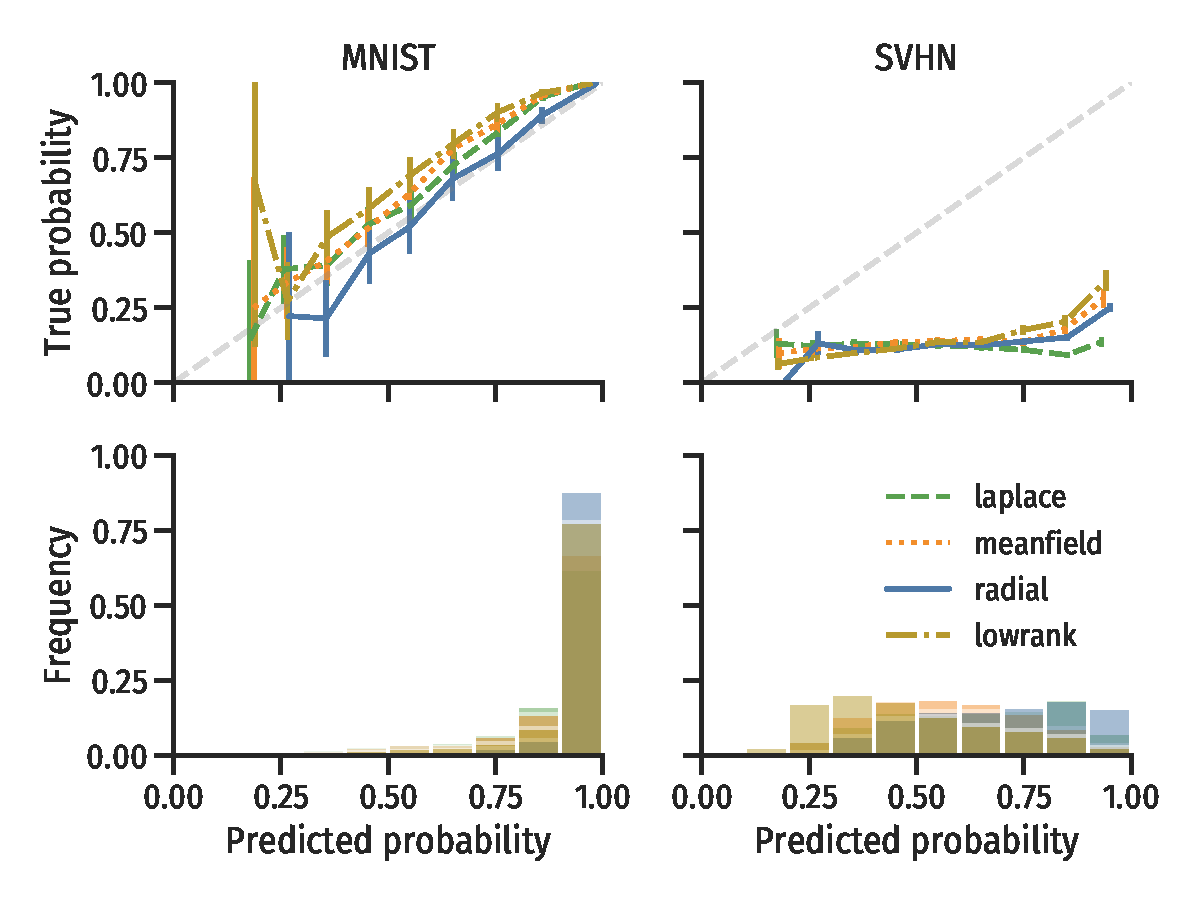
\includegraphics[width=\linewidth]{figures/MnistVI.pdf}
    \caption{Caption}
    \label{fig:cross-calibration}
\end{figure}
\begin{figure}
    \centering
    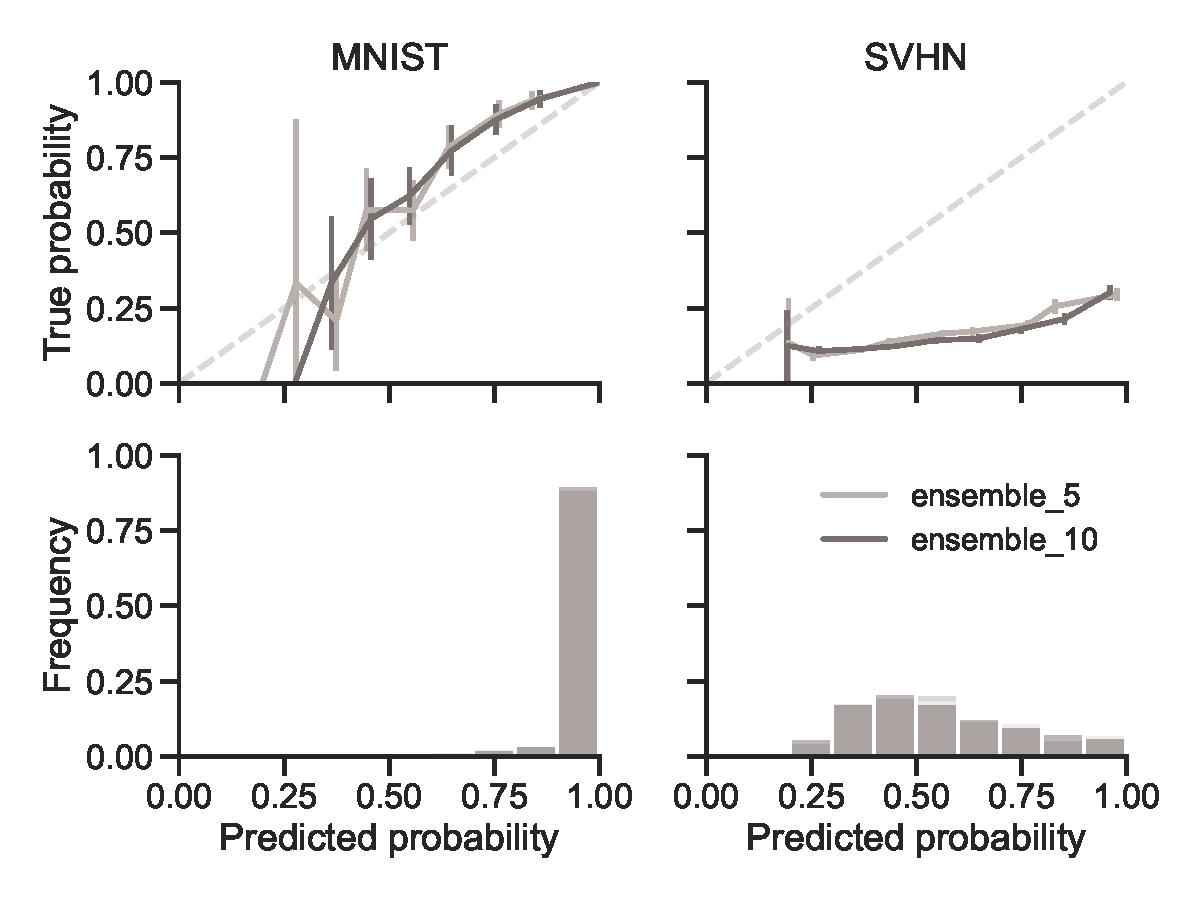
\includegraphics[width=\linewidth]{figures/MnistEnsembles.pdf}
    \caption{Caption}
    \label{fig:cross-calibration-ensemble}
\end{figure}
\begin{figure}
    \centering
    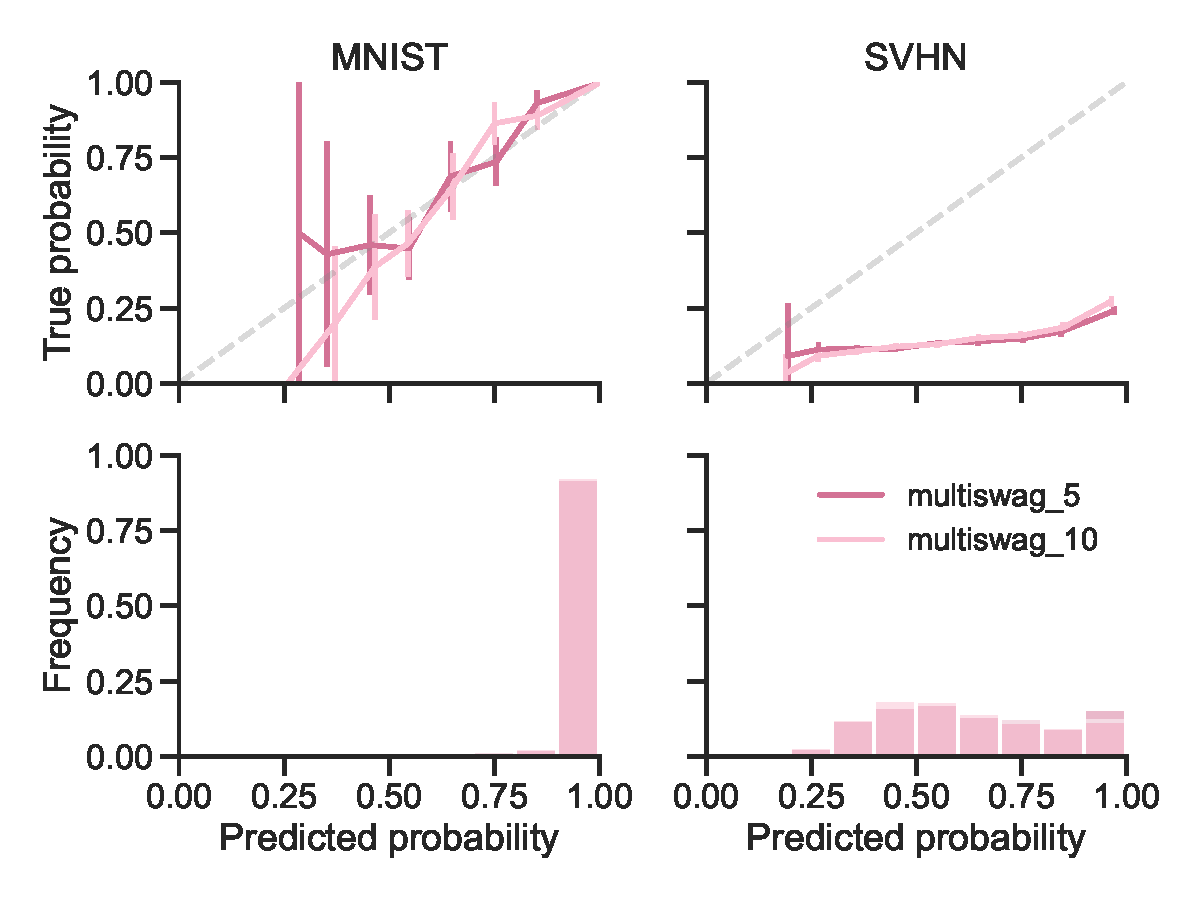
\includegraphics[width=\linewidth]{figures/MnistMultiSwag.pdf}
    \caption{Caption}
    \label{fig:cross-calibration-multiswag}
\end{figure}

\subsection{MURA}\label{ssec:mura}

% Method
\textcite{rajpurkar2017mura} introduced MURA, a musculoskeletal radiograph X-ray dataset for computer vision.
They trained a DenseNet with 169 layers~\cite{huang2017densely}
Due to computational constraints, we trained with the same dense neural network as in \cref{ssec:exp-mnist}.

% Results
%
\begin{figure}
    \centering
    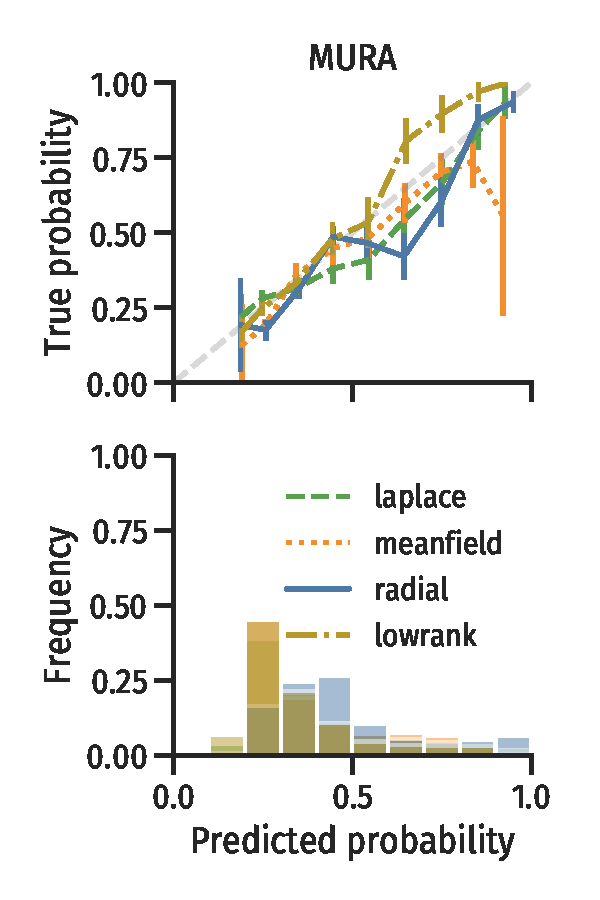
\includegraphics[width=0.55\linewidth]{figures/MuraVI.pdf}
    \caption{Caption}
    \label{fig:mura-cc-vi}
\end{figure}
\begin{figure}
    \centering
    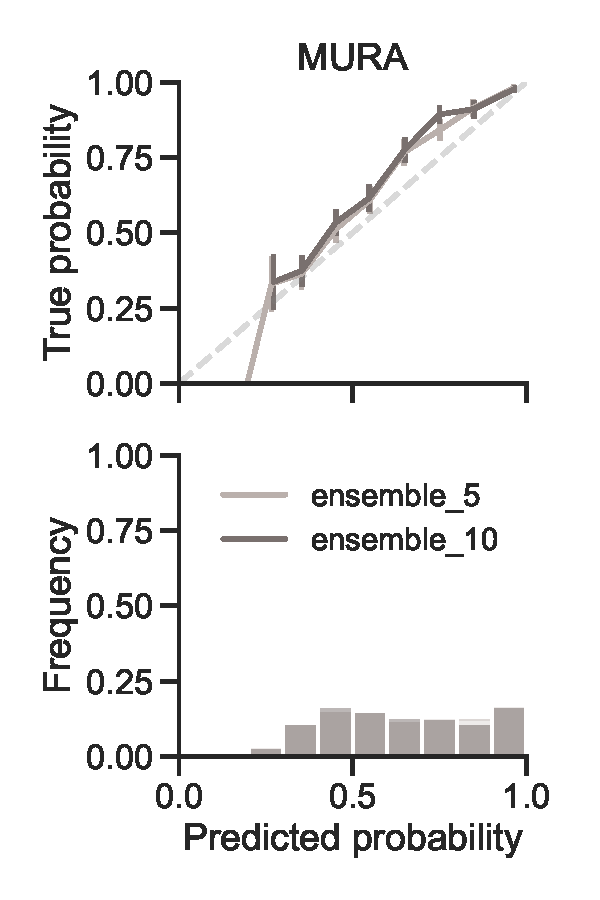
\includegraphics[width=0.55\linewidth]{figures/MuraEnsembles.pdf}
    \caption{Caption}
    \label{fig:mura-cc-ensembles}
\end{figure}
\begin{figure}
    \centering
    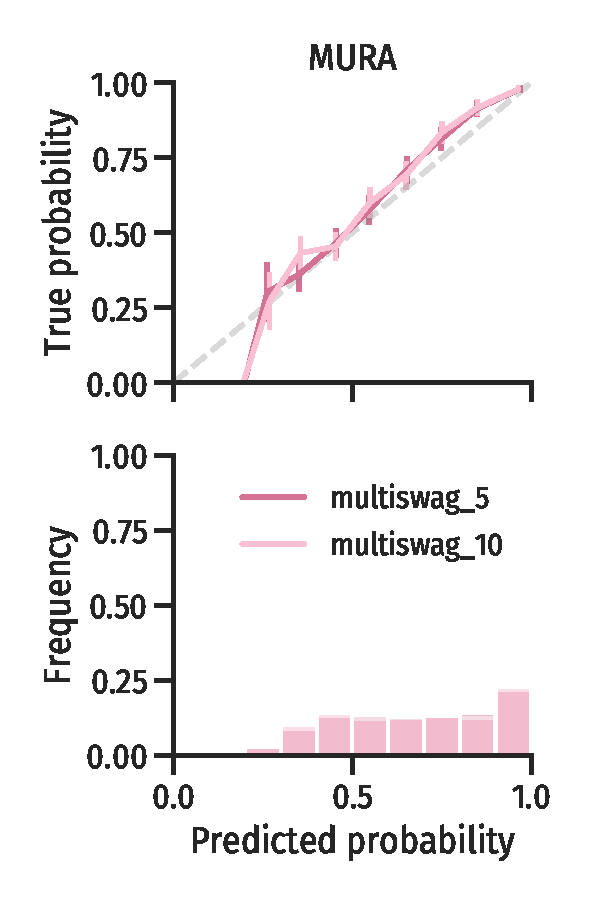
\includegraphics[width=0.55\linewidth]{figures/MuraMultiSwag.pdf}
    \caption{Caption}
    \label{fig:mura-cc-multiswag}
\end{figure}


Overall, ensembles performed very well on the classification tasks described in this paper --- both ones composed of deterministic models (deep ensembles) and those using SWAG posterior approximations (MultiSWAG).
However, there was not a significant difference in performance between the ensembles with 5 models and those with 10.
The training time of ensembles, if performed sequentially, scales linearly with the number of models in the ensemble.
Because of this, it can be beneficial to understand how the performance of an ensembly varies with the number of models.
\cref{fig:ensembles} shows that there is a clear performance improvement in going from a single model to an ensemble with two networks.
However, this performance gain quickly decays as the number of models is further increased; this may be caused by the simplicity of the MNIST classification problem.
%
\begin{figure}
    \centering
    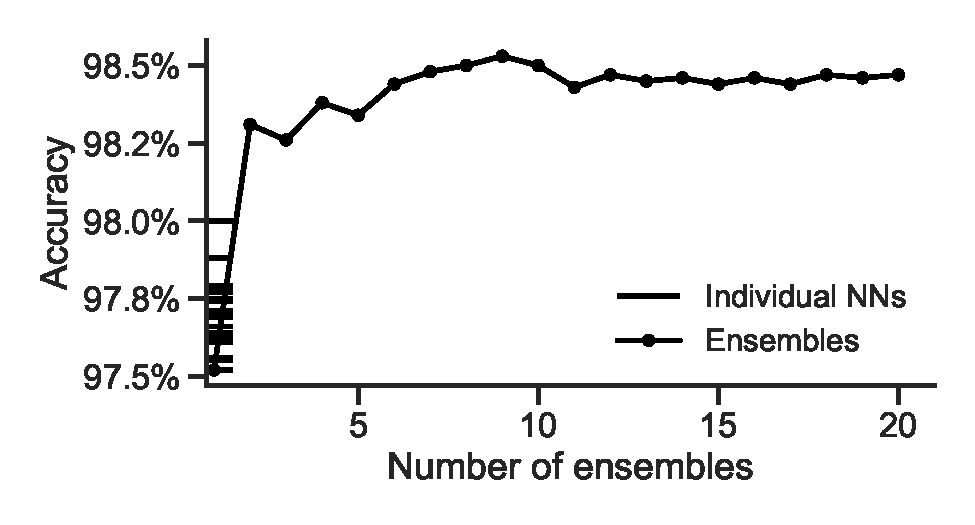
\includegraphics[width=\linewidth]{figures/ensemble_comparison.pdf}
    \caption{Ensembles with between one and twenty maximum likelihood NNs, trained on MNIST. We find that two ensembles have an increase of 0.8\% accuracy relative to a single neural network, with diminishing returns past this.}
    \label{fig:ensembles}
\end{figure}

\subsection{Active learning}

A convolutional neural network was trained using active learning on both the MNIST and MURA classification tasks.
%
\begin{figure*}
    \centering
    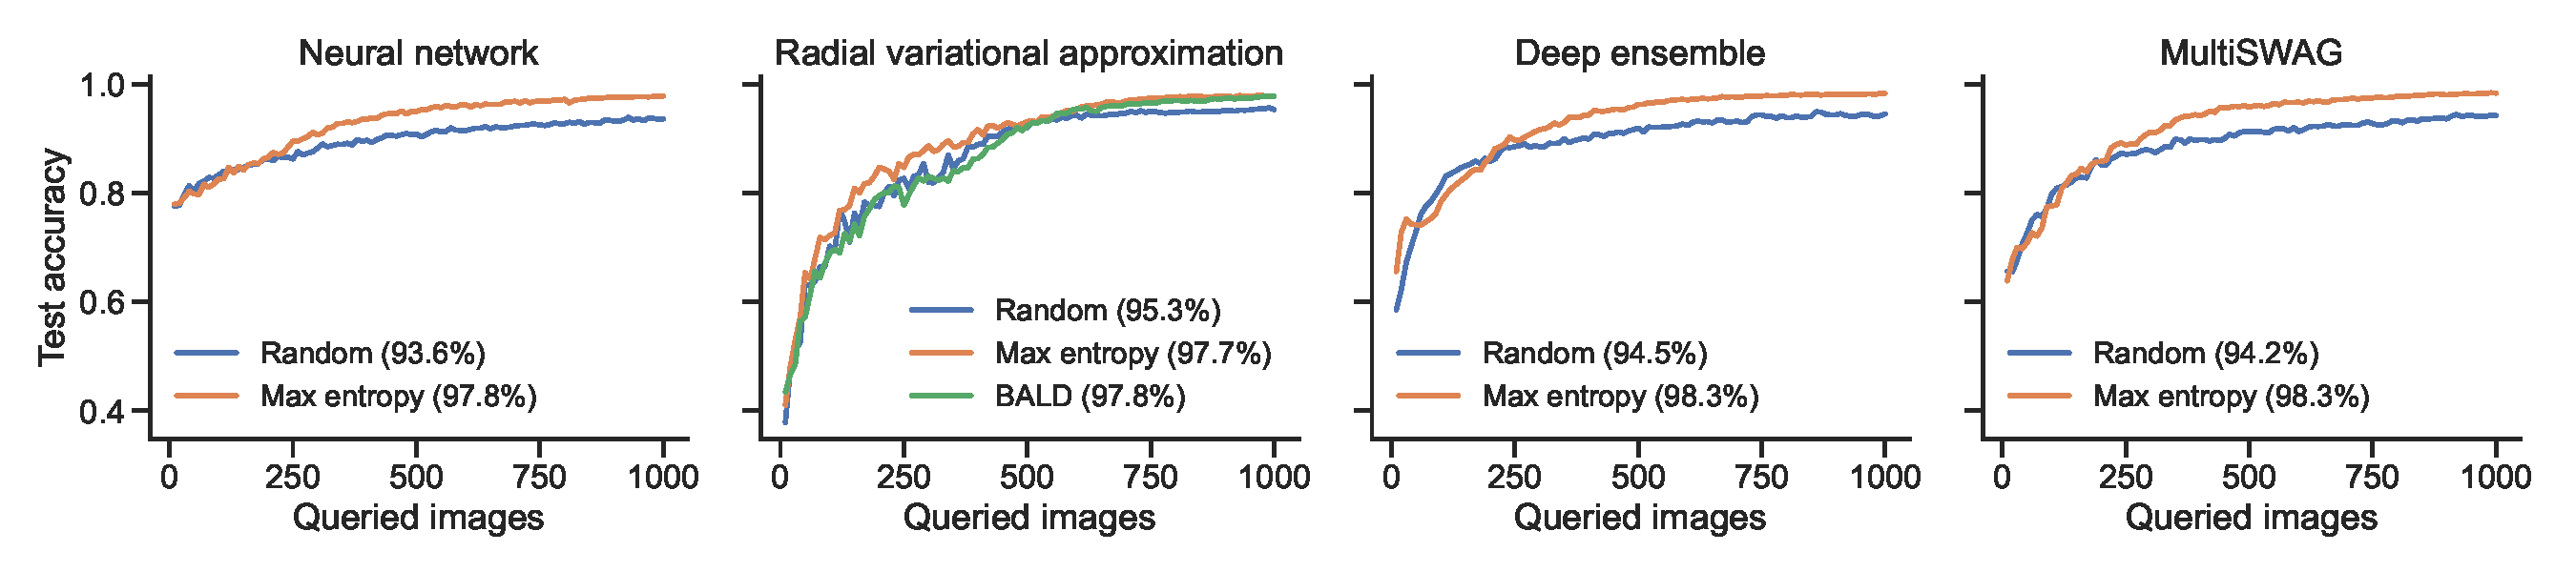
\includegraphics[width=\textwidth]{figures/active_comparison_mnist.pdf}
    \caption{Trained on MNIST.}
    \label{fig:active=mnist}
\end{figure*}
%
\begin{figure*}
    \centering
    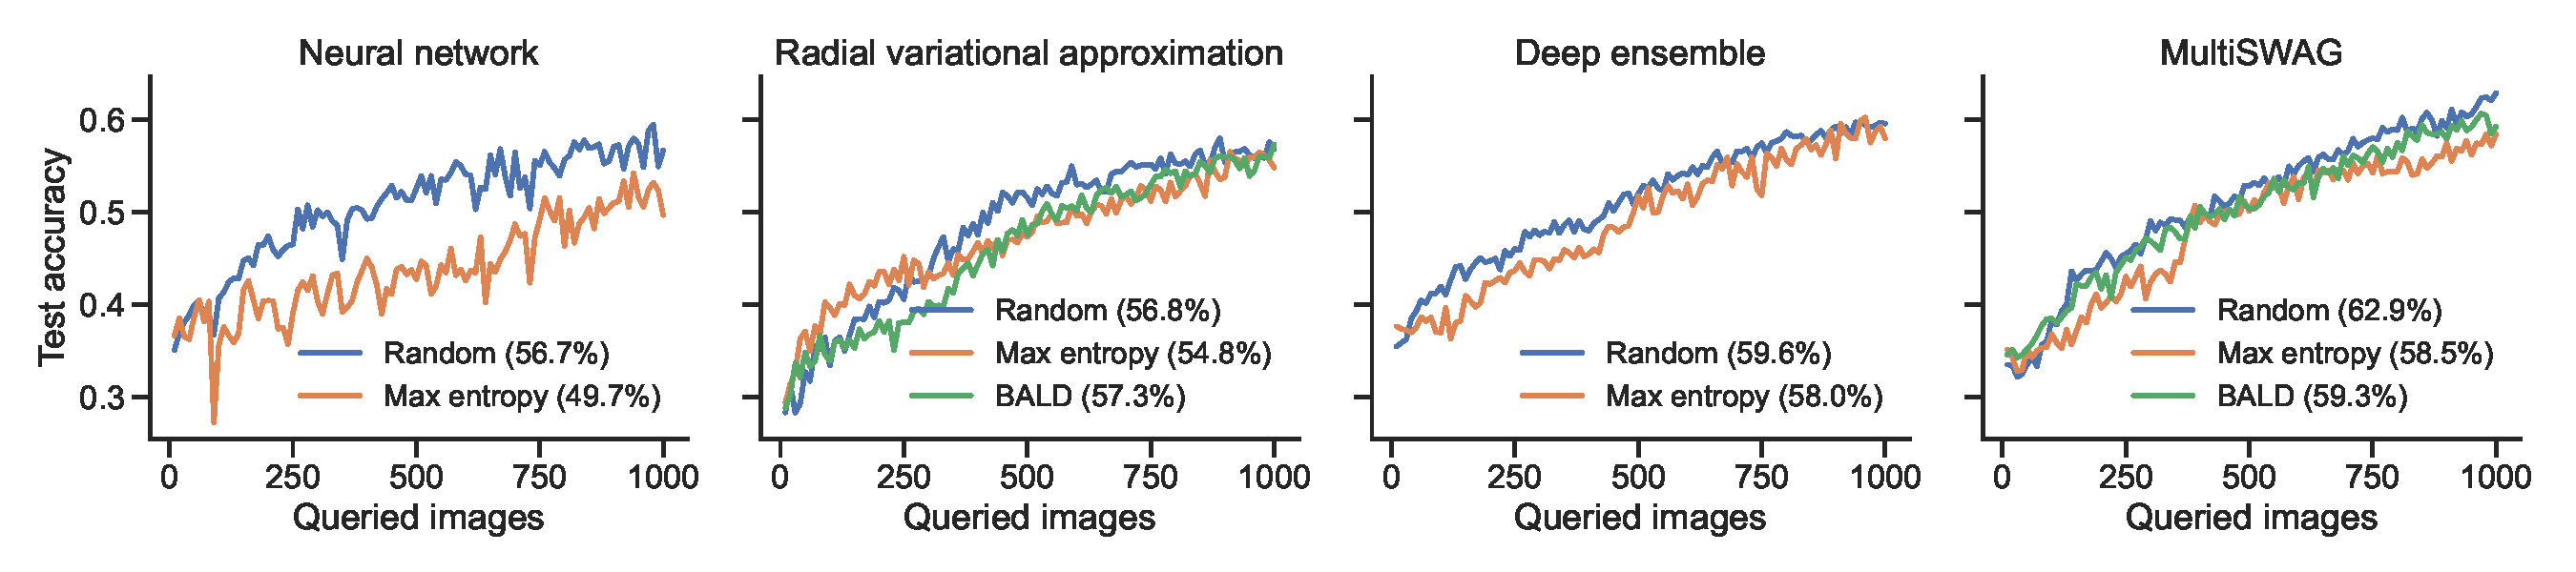
\includegraphics[width=\textwidth]{figures/active_comparison_mura.pdf}
    \caption{Trained on MURA.}
    \label{fig:active-mura}
\end{figure*}
\textcite{foong2020expressiveness} found that, for shallow mean-field VI BNNs, active learning doesn't show improvement over random acquisition.
This may be because VI for BNNs typically converge to a reasonable approximation of the mean faster than they approximate the variance.
This means that, since we start the active learning process on an untrained BNN, the initial iterations quantify uncertainty poorly and therefore their predictive entropy has little value.

\section{Conclusion}

% Summary and key results

% Outlook and future developments
\textbf{Ideas for experiments}
\begin{enumerate}
    \item Is it better to train an Nx bigger neural network, or to ensemble N neural networks? Mind you, deep ensembles have the advantage of easy parallelization.
    \item See what happens with a mean field when you increase width or depth
    \item See what happens with VI if you increase the size of the model, over-parameterise
\end{enumerate}

\printbibliography

\clearpage
\onecolumn
\appendix
\section{Appendix}
\begin{table}[h]
    \centering
    \begin{tabular}{llrrrrrrr}
Inference & Evaluated on & NLL & Accuracy & AUROC & Avg. Conf. & Avg. Conf. - & Avg. Conf. + & ECE \\
Ensemble@5 & MNIST & -0.975 & 0.984 & 1.000 & 0.983 & 0.712 & 0.987 & 0.007 \\
Ensemble@10 & MNIST & -0.975 & 0.984 & 1.000 & 0.982 & 0.667 & 0.987 & 0.002 \\
MultiSWAG@5 & MNIST & -0.970 & 0.984 & 1.000 & 0.976 & 0.635 & 0.982 & 0.009 \\
MultiSWAG@10 & MNIST & -0.970 & 0.985 & 1.000 & 0.976 & 0.626 & 0.981 & 0.009 \\
Radial & MNIST & -0.879 & 0.928 & 0.995 & 0.898 & 0.610 & 0.920 & 0.030 \\
Mean-field & MNIST & -0.465 & 0.577 & 0.903 & 0.464 & 0.171 & 0.679 & 0.113 \\
Low-rank & MNIST & -0.848 & 0.926 & 0.995 & 0.860 & 0.490 & 0.889 & 0.066 \\
Laplace & MNIST & -0.839 & 0.975 & 1.000 & 0.844 & 0.438 & 0.854 & 0.131 \\
ML & MNIST & -0.976 & 0.977 & 0.999 & 0.992 & 0.841 & 0.996 & 0.033 \\
\end{tabular}

    \caption{Trained on MNIST.}
    \label{tab:mnist}
\end{table}
\begin{table}[h]
    \centering
    \begin{tabular}{llrrrrrrr}
\toprule
        Type & Evaluated on &     NLL &  Accuracy &  AUROC &  Avg. Conf. &  Avg. Conf. - &  Avg. Conf. + &    ECE \\
\midrule
  Ensemble@5 &         MURA & -0.5614 &    0.7094 & 0.9380 &      0.6503 &        0.4915 &        0.7154 & 0.0592 \\
 Ensemble@10 &         MURA & -0.5587 &    0.7160 & 0.9394 &      0.6436 &        0.4852 &        0.7064 & 0.0724 \\
 MultiSWAG@5 &         MURA & -0.5916 &    0.7188 & 0.9409 &      0.6847 &        0.5149 &        0.7512 & 0.0342 \\
MultiSWAG@10 &         MURA & -0.5895 &    0.7207 & 0.9423 &      0.6788 &        0.5072 &        0.7453 & 0.0420 \\
      Radial &         MURA &  1.4535 &    0.4376 & 0.7956 &      0.4755 &        0.4058 &        0.5650 & 0.0618 \\
  Mean-field &         MURA &  1.7662 &    0.3519 & 0.6842 &      0.3935 &        0.3460 &        0.4809 & 0.0480 \\
    Low-rank &         MURA &  1.6063 &    0.3716 & 0.7499 &      0.3582 &        0.2989 &        0.4584 & 0.0231 \\
     Laplace &         MURA &  1.6759 &    0.3835 & 0.7003 &      0.4034 &        0.3486 &        0.4914 & 0.0481 \\
          ML &         MURA &  1.2315 &    0.5508 & 0.8617 &      0.5203 &        0.4375 &        0.5878 & 0.0349 \\
         MAP &         MURA &  1.7103 &    0.3585 & 0.6732 &      0.4155 &        0.3516 &        0.5298 & 0.0601 \\
\bottomrule
\end{tabular}

    \caption{Trained on MURA.}
    \label{tab:mura}
\end{table}

\end{document}
